\chapter{Preliminary}
%%%%%%%%%%%%%%%%%%%%%%%%%%%%%%%%%%%%%%%%%%%%%%%%%%%%%%%%%%%%%%%%%%%%%%%%%%%%%%%%

In this chapter, The notation used throughout this thesis, the modeling of multi-link aerial robots, and the external wrench estimation method will be introduced. In the modeling part, two types of multi-link aerial robots will be presented. One is the underactuated multi-link aerial robot Hydrus Xi, which can achieve 2D deformation while retaining the overall actuation of a conventional quadrotor. The other is the overactuated multi-link aerial robot DRAGON, which can deform in a 3D workspace. The basic constructions, dynamics and allocation modeling processes will be introduced.


\section{Notation}
In this thesis, we denote scalars by regular font $x \in \mathbb{R}$, vectors by bold lowercase $\boldsymbol{x} \in \mathbb{R}^n$, and matrices by bold uppercase $\boldsymbol{X} \in \mathbb{R}^{m \times n}$. A vector expressed in frame $\{A\}$ is written as $^A\boldsymbol{p}$, and the rotation matrix from frame $\{A\}$ to frame $\{B\}$ is denoted as $^A\boldsymbol{R}_B$.
Also, $\{W\}$ represents the world frame, and $\{C\}$ represents the CoG frame. For each link $i\in\{1,2,3,4\}$, $\{F_i\}$ and $\{G_i\}$ denote the thrust frame and gimbal roll frame of the corresponding gimbal module, while $\{L_i\}$ denotes the corresponding link frame.

%%%%%%%%%%%%%%%%%%%%%%%%%%%%%%%%%%%%%%%%%%%%%%%%%%%%%%%%%%%%%%%%%%%%%%%%%%%%%%%%

\section{Modeling of Multi-Link Aerial Robots}

\subsection{General Description of Multi-Link Aerial Robots}
The multi-link aerial robots consist of multiple serially connected links for deformation. Two typical multi-link aerial robots are shown in Fig.~\ref{fig:multi-link}. The relative angles between the adjacent links can be changed through joint actuation, enabling robotic arm-like movements in the air. To realize the dexterous aerial motion, rotors are arranged on the gimbal modules, which can change the thrust direction of the rotors depending on the gimbal types, thereby achieving vectoring thrust. Each link is equipped with one gimbal module. The thrust direction of each rotor can be adjusted by the gimbal module to maintain stable flight and generate the required wrench for aerial manipulation. In particular, the required thrust direction varies with the joint configuration, even when the desired flight condition remains unchanged.


\subsection{Dynamic Model}

Using the notation defined above, the dynamics of the multi-link aerial robots at their CoG, derived from the Newton--Euler equations, are given by:
\begin{subequations}
\label{eq:dynamics}
\begin{align}
    m(^W\!\ddot{\boldsymbol{p}}+\boldsymbol{g})&= {^W\!\boldsymbol{f}_{cmd}} + {^W\!\boldsymbol{f}_{ext}}, \\[2pt]
    \boldsymbol{I}{^C\!\dot{\boldsymbol{\omega}}}+{^C\!\boldsymbol{\omega}} \times \boldsymbol{I}{^C\!\boldsymbol{\omega}}&={^C\!\boldsymbol{\tau}_{cmd}} + {^C\!\boldsymbol{\tau}_{ext}},
\end{align}
\end{subequations}
where $m$ is the total mass, $\boldsymbol{I}$ is the total inertia matrix expressed in frame $\{C\}$, $^W\boldsymbol{p}$ is the position of the oringinal point of  the CoG frame $\{C\}$ in the world frame $\{W\}$, $^{C}\boldsymbol{\omega}$ is the angular velocity of the CoG frame $\{C\}$ expressed in frame $\{C\}$, $\boldsymbol{g}$ is the gravitational acceleration, ${^W\!\boldsymbol{f}_{cmd}}$, ${^C\!\boldsymbol{\tau}_{cmd}}$ and ${^W\!\boldsymbol{f}_{ext}}$, ${^C\!\boldsymbol{\tau}_{ext}}$ denote the command force and torque, and the external force and torque, respectively. Since the joint angles and thrust directions vary during motion, the inertia matrix is configuration dependent and may vary accordingly. Here, we consider the multi-link aerial robot as a quasi-static system, meaning that the variations in the inertia matrix caused by joint and thrust-vectoring motions are negligible within a single control period \cite{zhao_2021_singularity, zhao_2023_versatile}.


\begin{figure}[t]
    \centering
    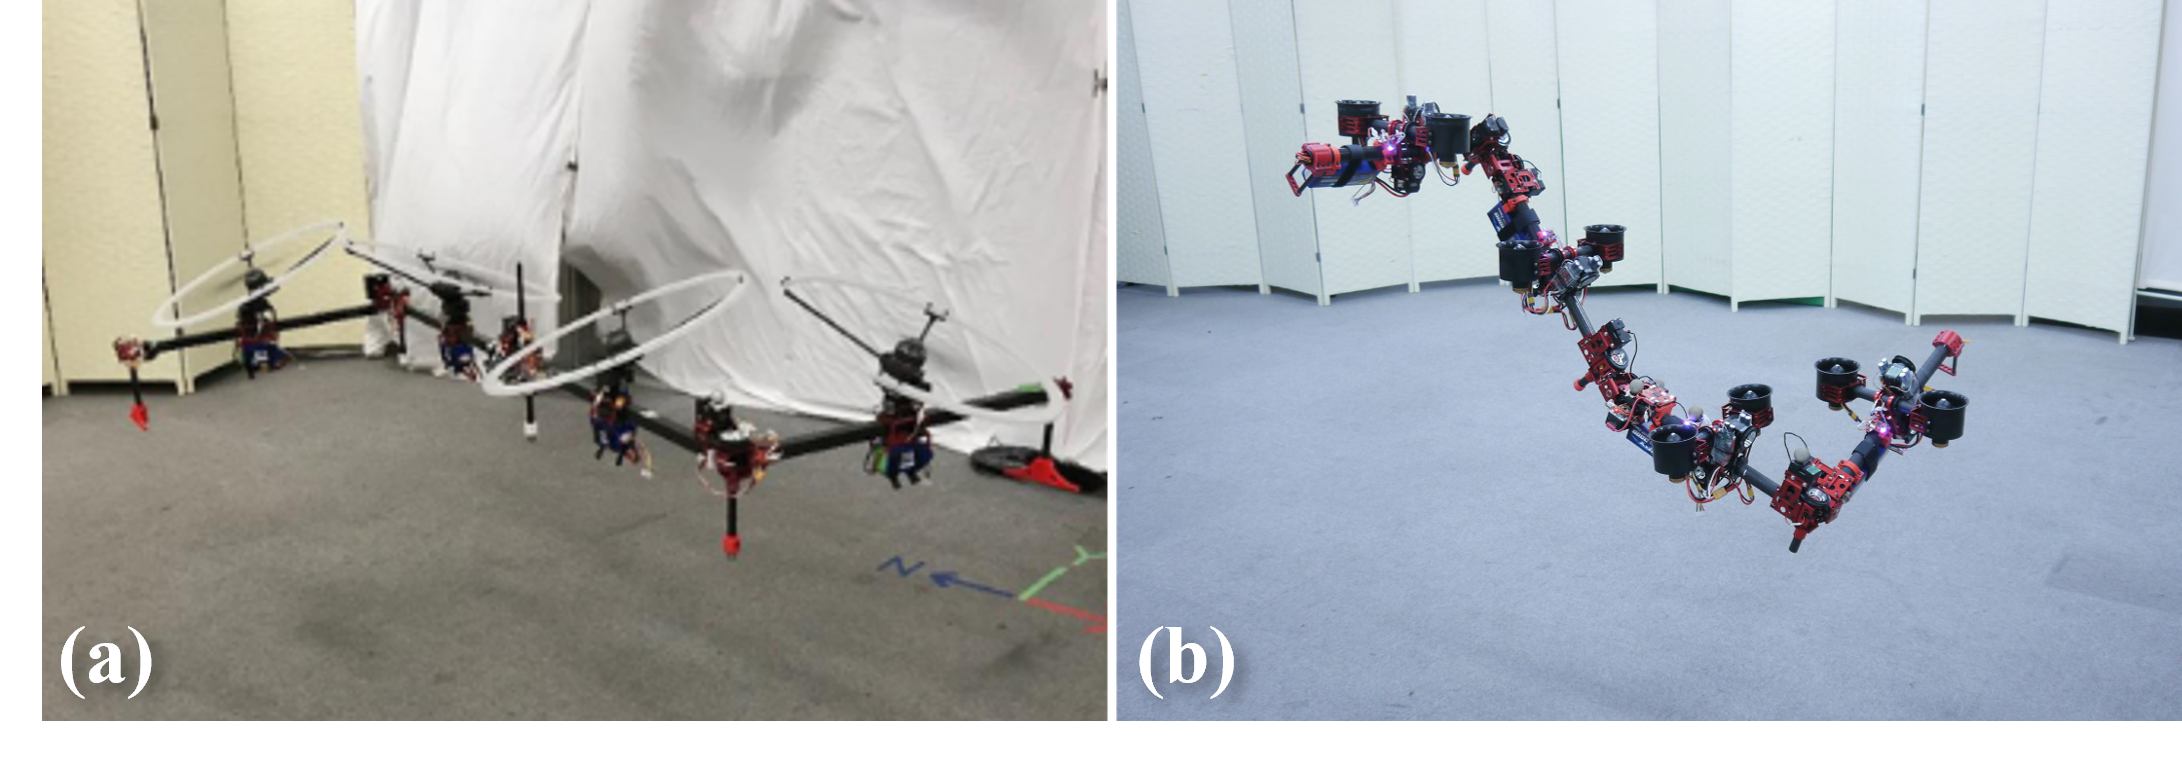
\includegraphics[trim={0cm 0cm 0cm 0cm}, clip, width=\linewidth]{figures/chapter2/multi-link.png}
    \caption{Photographs of the multi-link aerial robots. (a): underactuated multi-link aerial robot Hydrus Xi \cite{zhao_2021_singularity}. (b): overactuated mutli-link aerial robot DRAGON \cite{zhao_2018_design}.}
    \label{fig:multi-link}
\end{figure}

\subsection{Allocation}
The command force ${^W\boldsymbol{f}_{cmd}}$ and the command torque ${^{C}\boldsymbol{\tau}_{cmd}}$ are obtained by aggregating the contributions of the rotors mounted on the gimbal modules, whose individual forces and torques are expressed in frame $\{C\}$. We compute each module's contribution as follows:
\begin{equation}
\label{eq:allocation for force}
    {^C\!\boldsymbol{f}_i}=\lambda_i^C\!\boldsymbol{R}_{F_i}\boldsymbol{b}_3,
\end{equation}

\begin{equation}
\begin{aligned}
\label{eq:allocation for torque}
    {^C\!\boldsymbol{\tau}_i}&=^C\!\!\boldsymbol{p}_{F_i}\times^C\!\!\boldsymbol{f}_i+\kappa_i ^C\!\boldsymbol{f}_i\\
    &=\lambda_i(^{C}\boldsymbol{\hat{p}}_{F_i}+\kappa_i\boldsymbol{E}_3)^C\boldsymbol{R}_{F_i}\boldsymbol{b}_3.
\end{aligned}
\end{equation}
Here, $i\in\{1,2,3,4\}$ since the multi-link aerial robots considered in this thesis consist of four links. The joint angles and thrust directions determine $^{C}\boldsymbol{R}_{F_i}\in \mathbb{R}^{3\times3}$ and $^{C}\boldsymbol{p}_{F_i}\in \mathbb{R}^3$, which denote the rotation matrix and the position vector of the rotor frame $\{F_i\}$ with respect to the CoG frame $\{C\}$. The rotor frame $\{F_i\}$ is attached to the rotor mount, and the thrust force $\lambda_i$ is along the $z$ axis of $\{F_i\}$. The vector $\boldsymbol{b}_3 = \begin{bmatrix}0 & 0 & 1\end{bmatrix}^{\mathrm{T}}$ is a unit vector and $\kappa_i$ is the coefficient associated with the rotor drag moment. The operator $\hat{\cdot}$ converts a vector into a skew-symmetric matrix, and $\boldsymbol{E}_3$ denotes the $3 \times 3$ identity matrix. 

Using \eqref{eq:allocation for force} and \eqref{eq:allocation for torque}, the mapping from the thrust vector $\boldsymbol{\lambda} = \begin{bmatrix}\lambda_1 & \lambda_2 & \lambda_3&\lambda_4\end{bmatrix}^{\mathrm{T}}$ to the command wrench is given by:
\begin{equation}
\label{eq:allocation for wrench}
^C\!\boldsymbol{w}_{cmd}
=
\begin{pmatrix}
^C\!\boldsymbol{f}_{cmd} \\
^C\!\boldsymbol{\tau}_{cmd}
\end{pmatrix}
=
\sum_{i=1}^{4}
\begin{pmatrix}
^C\!\boldsymbol{f}_i \\
^C\!\boldsymbol{\tau}_i
\end{pmatrix} 
=\begin{pmatrix}
\boldsymbol{Q}_t \\
\boldsymbol{Q}_r
\end{pmatrix}\boldsymbol{\lambda},
\end{equation}
where $\boldsymbol{Q}_t \in \mathbb{R}^{3\times4}$ and $\boldsymbol{Q}_r\in \mathbb{R}^{3\times4}$ denote the translational and rotational components of the allocation matrix, respectively. The command force in the world frame can be obtained by $^W\!\boldsymbol{f}_{cmd} = ^W\!\!\!\boldsymbol{R}_C{}^C\!\boldsymbol{f}_{cmd}$.

In this thesis, the allocation matrices $\boldsymbol{Q}_t$ and $\boldsymbol{Q}_r$ depend on the joint angles and thrust directions. We use the optimization method introduced in \cite{zhao_2021_singularity} or an iterative solution using gradients based on an optimization method introduced in \cite{zhao_2023_versatile} to calculate the thrust directions and the gimbal angles automatically. 


\subsection{Underactuated Configuration: Hydrus Xi}
The underactuated multi-link aerial robot Hydrus Xi \cite{zhao_2021_singularity} is shown in Fig.~\ref{fig:hydrus_model}. The platform consists of four links, each of which carries an independent gimbal module. The robot employs a serial-link structure with one rotational degree of freedom per joint, whose joint axes are aligned in parallel. Here, $q_i$ is used to represent the $i$th joint angle. Each gimbal module features a fixed tilt angle $\beta$ and a 1-DoF yaw rotation mechanism to vector the thrust direction. The corresponding rotation angle, referred to as the vectoring angle, is denoted by $\psi_i$. The design of the gimbal module was originally developed in \cite{anzai_2019_design}. Besides the joint angles, Hydrus Xi has eight actuation inputs: four rotor thrusts $\boldsymbol\lambda$ and four vectoring angles $\boldsymbol\psi$. However, to maximize the possible torque generated under the current configuration, the vectoring angles $\boldsymbol\psi$ are automatically adjusted through an optimization method \cite{zhao_2021_singularity}. Therefore, only the four rotor thrusts remain as direct control inputs, making Hydrus Xi an underactuated system.


\begin{figure}[t]
    \centering
    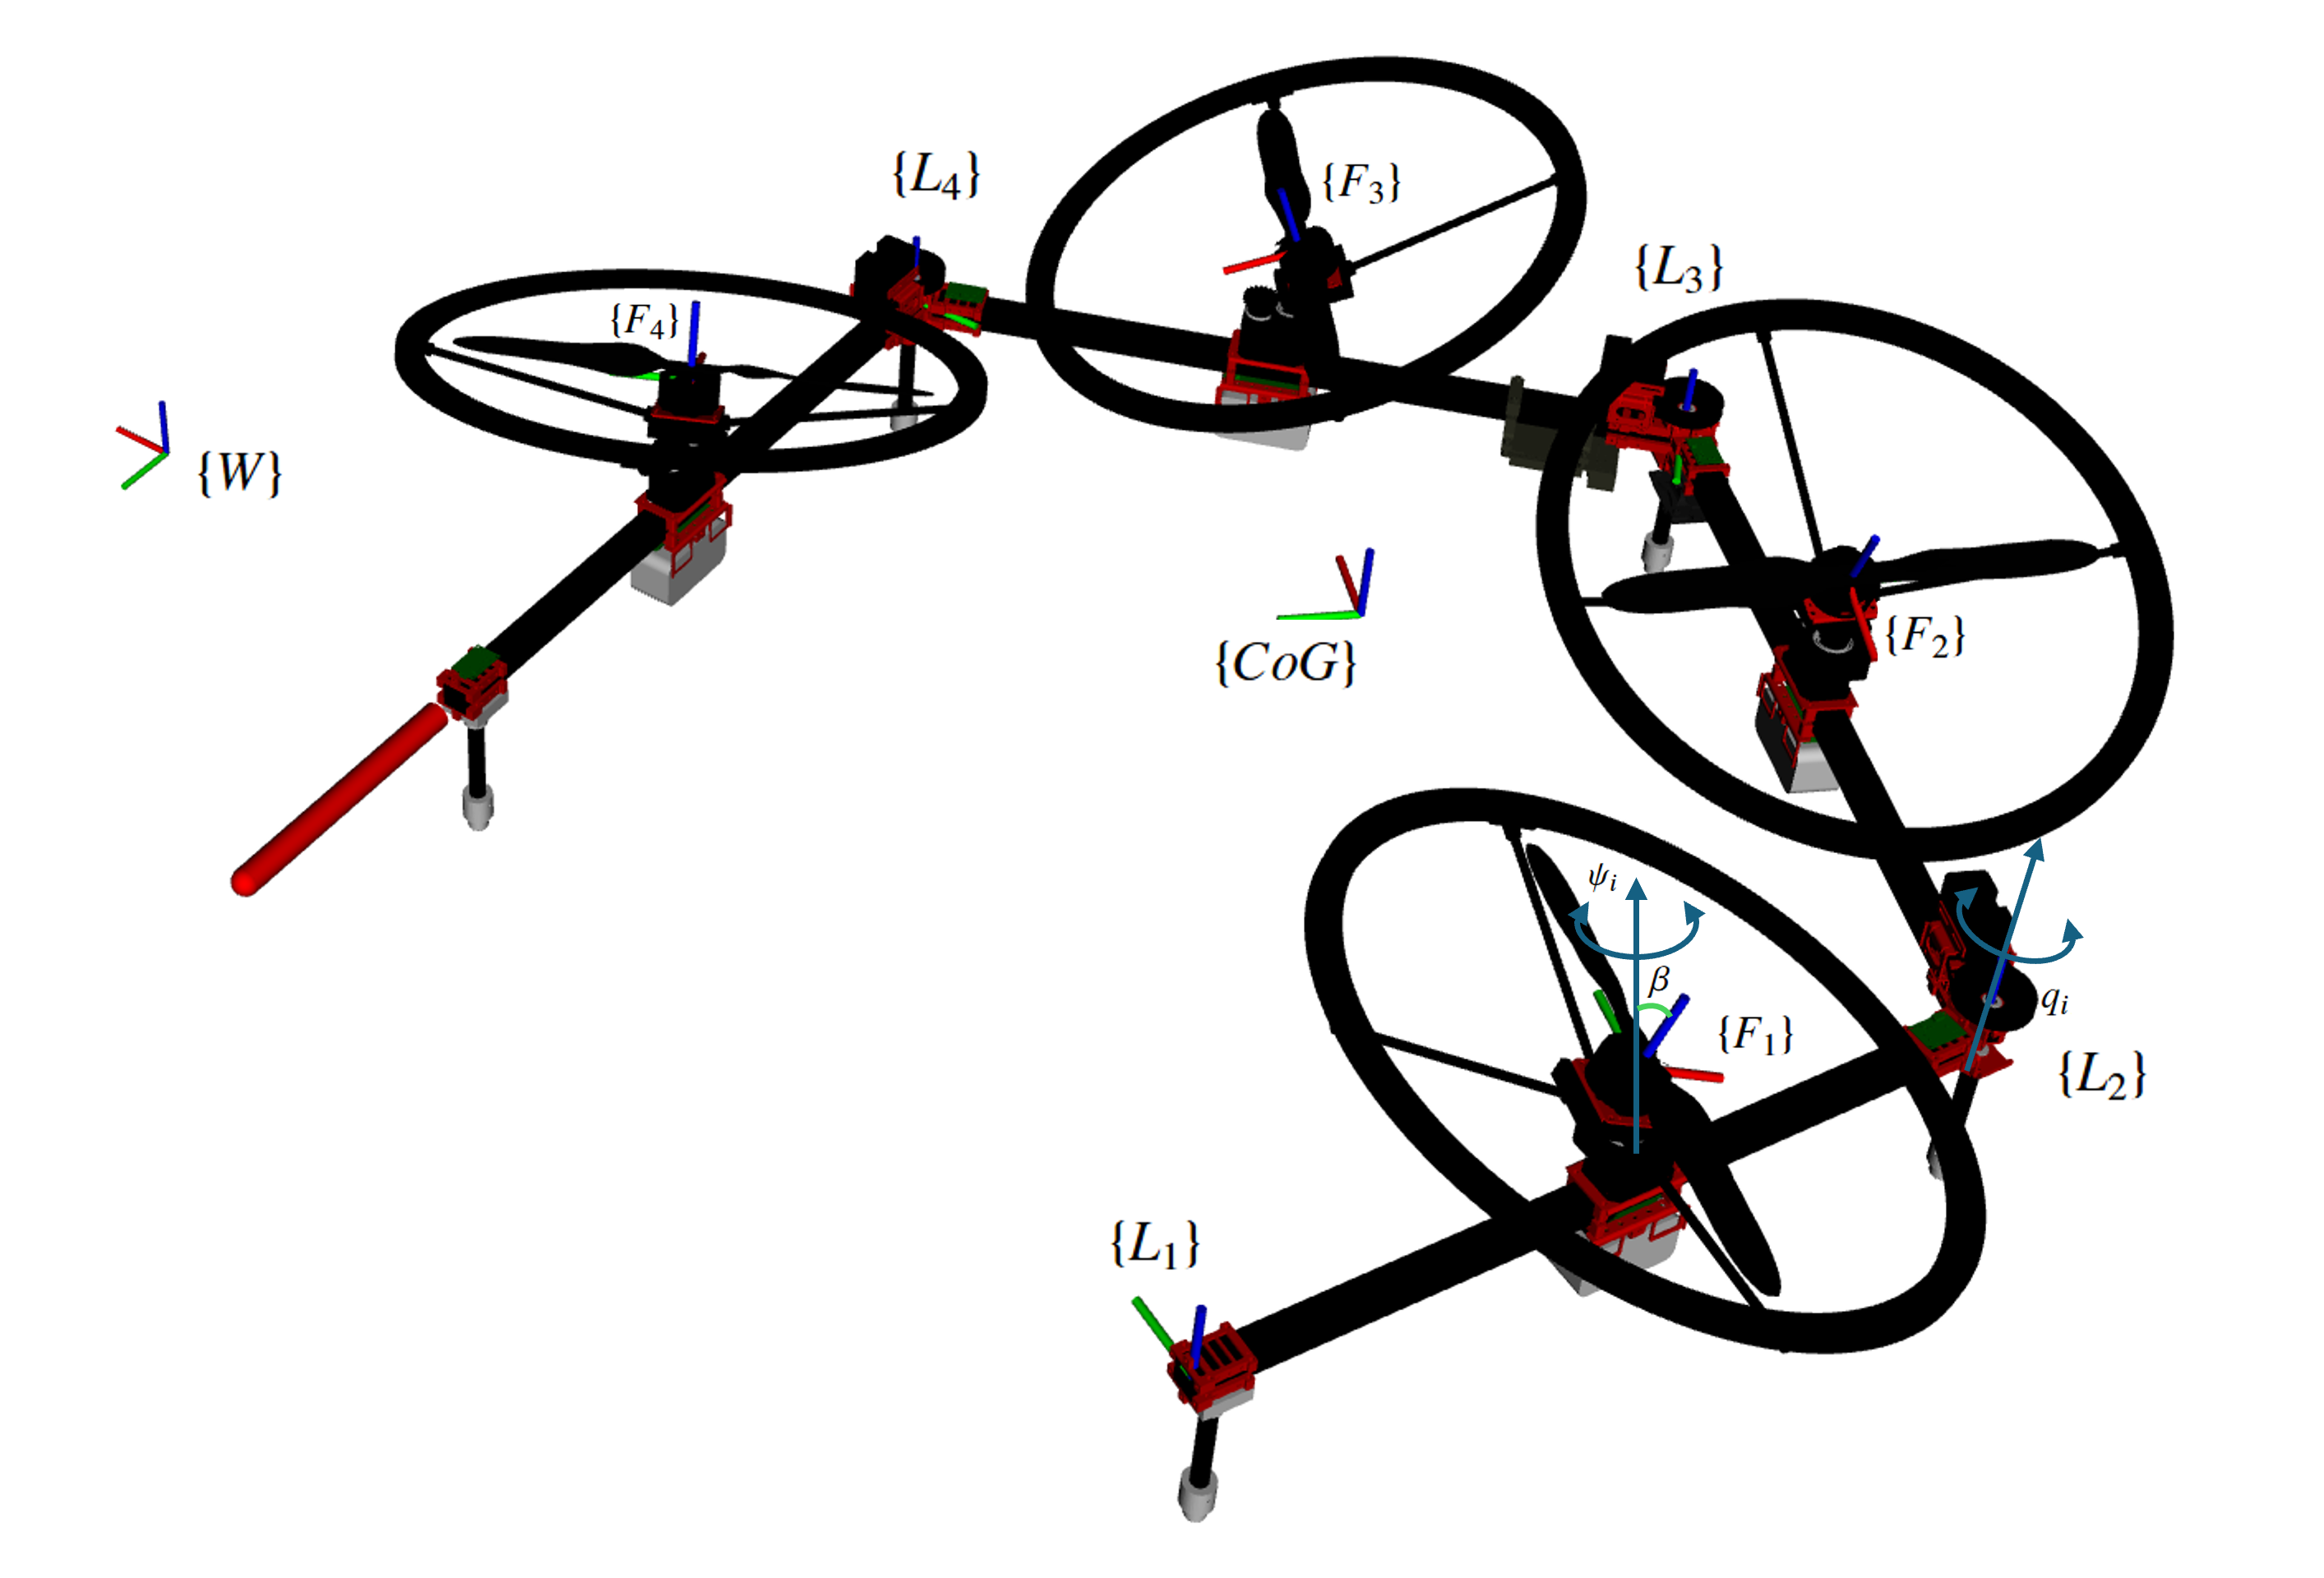
\includegraphics[trim={0cm 0cm 0cm 0cm}, clip, width=\linewidth]{figures/chapter2/hydrus_model.png}
      \caption{Model of the underactuated multi-link aerial robot Hydrus Xi. $\{L_i\}$ denotes the link frame, while $\{F_i\}$ denotes the thrust frame whose $z$ axis is aligned with the thrust direction. The tilt angle between $z$ axes of $\{L_i\}$ and $\{F_i\}$ is $\beta$, and the vectoring angle is $\psi_i$. }
    \label{fig:hydrus_model}
\end{figure}


Note that the transform from $\{C\}$ to $\{F_i\}$ changes due to the joint angles $q_i$ and the vectoring angles $\psi_i$. Therefore, the command equations (\ref{eq:allocation for force}), (\ref{eq:allocation for torque}) and (\ref{eq:allocation for wrench}) can be rewritten as

\begin{equation}
\label{eq:allocation for force hydrus}
    {^C\!\boldsymbol{f}_i}=\lambda_i^C\!\boldsymbol{R}_{F_i}(\boldsymbol{q},\boldsymbol{\psi})\boldsymbol{b}_3,
\end{equation}

\begin{equation}
\begin{aligned}
\label{eq:allocation for torque hydrus}
    {^C\!\boldsymbol{\tau}_i}&=^C\!\!\boldsymbol{p}_{F_i}(\boldsymbol{q},\boldsymbol{\psi})\times^C\!\!\boldsymbol{f}_i+\kappa_i ^C\!\boldsymbol{f}_i\\
    &=\lambda_i(^{C}\boldsymbol{\hat{p}}_{F_i}(\boldsymbol{q},\boldsymbol{\psi})+\kappa_i\boldsymbol{E}_3)^C\!\boldsymbol{R}_{F_i}(\boldsymbol{q},\boldsymbol{\psi})\boldsymbol{b}_3,
\end{aligned}
\end{equation}

\begin{equation}
\label{eq:allocation for wrench hydrus}
^C\!\boldsymbol{w}_{cmd}
=
\begin{pmatrix}
^C\!\boldsymbol{f}_{cmd} \\
^C\!\boldsymbol{\tau}_{cmd}
\end{pmatrix}
=
\sum_{i=1}^{4}
\begin{pmatrix}
^C\!\boldsymbol{f}_i \\
^C\!\boldsymbol{\tau}_i
\end{pmatrix} 
=\begin{pmatrix}
\boldsymbol{Q}_t(\boldsymbol{q},\boldsymbol{\psi}) \\
\boldsymbol{Q}_r(\boldsymbol{q},\boldsymbol{\psi})
\end{pmatrix}\boldsymbol{\lambda},
\end{equation}
where $\boldsymbol{Q}_t(\boldsymbol{q},\boldsymbol{\psi}) $ and $\boldsymbol{Q}_r(\boldsymbol{q},\boldsymbol{\psi})$ are functions of the joint angles $\boldsymbol q$ and vectoring angles $\boldsymbol\psi$.



\subsection{Overactuated Configuration: DRAGON}
The overactuated multi-link aerial robot DRAGON \cite{zhao_2018_design, zhao_2023_versatile} is shown in Fig.~\ref{fig:dragon_model}. The platform also consists of four links, each of which is equipped with an independent gimbal module. The robot employs a serial-link structure with two rotational degrees of freedom between adjacent links, realized by two orthogonal rotational joints. Here, $q_i$ is used to represent the $i$th joint angle. Each gimbal module has two gimbal angles, $\phi_i$ and $\theta_i$, which provide two degrees of freedom for changing the thrust direction relative to the corresponding link. More details of the robot structure can be found in \cite{zhao_2018_design}. In DRAGON's case, there are 12 actuation inputs excluding the joint angles, including four rotor thrusts $\boldsymbol{\lambda}$, four gimbal roll angles $\boldsymbol{\phi}$, and four gimbal pitch angles $\boldsymbol{\theta}$. All of them need to be determined as control inputs. With these redundant actuation inputs, DRAGON is an overactuated system.



\begin{figure}[t]
    \centering
    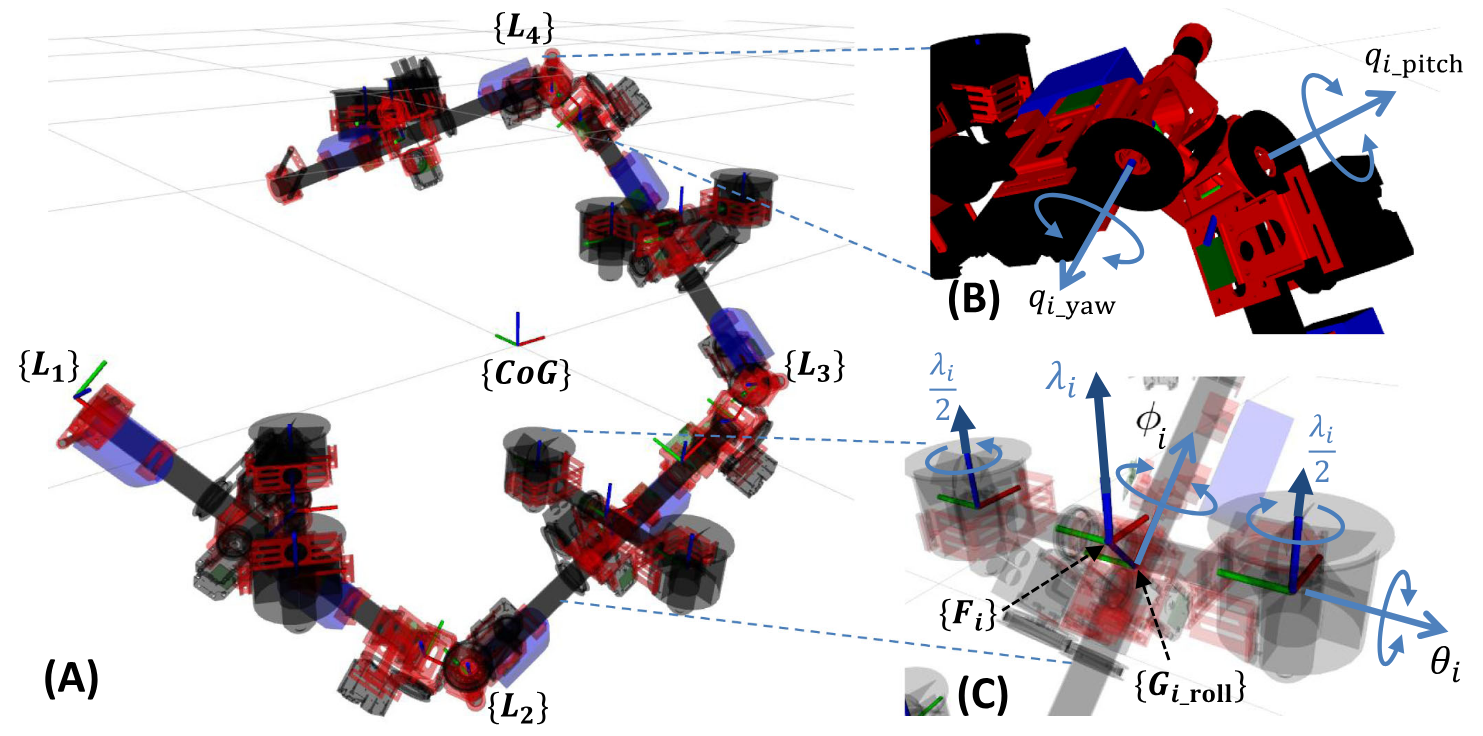
\includegraphics[trim={0cm 0cm 0cm 0cm}, clip, width=\linewidth]{figures/chapter2/dragon_model.png}
    \caption{Model of the overactuated multi-link aerial robot DRAGON. (a) Kinematic model of DRAGON, with $\{L_i\}$ denoting the link frame. (b) Two-DoF joint module with orthogonal yaw and pitch axes ($q_{i\_yaw}$, $q_{i\_pitch}$). (c) Two-DoF thrust-vectoring apparatus with gimbal angles $\theta_i$ and $\phi_i$. $\{G_i\}$ denotes the intermediate frame (gimbal roll frame) after the $\phi_i$ rotation, while $\{F_i\}$ denotes the thrust frame whose $z$ axis is aligned with the thrust direction.}
    \label{fig:dragon_model}
\end{figure}




In DRAGON's case, the command equations (\ref{eq:allocation for force}), (\ref{eq:allocation for torque}) and (\ref{eq:allocation for wrench}) can be rewritten as 

\begin{equation}
\label{eq:allocation for force dragon}
    {^C\!\boldsymbol{f}_i}=\lambda_i^C\!\boldsymbol{R}_{L_i}(\boldsymbol{q})^{L_i}\boldsymbol{R}_{G_i}(\phi_i)^{G_i}\boldsymbol{R}_{F_i}(\theta_i)\boldsymbol{b}_3=\lambda_i^{C}\!\boldsymbol{u}_i.
\end{equation}

\begin{equation}
\label{eq:allocation for torque dragon}
    {^C\!\boldsymbol{\tau}_i}=\lambda_i^{C}\!\boldsymbol{p}_{F_i}(\boldsymbol{q}, \phi_i ) \times ^{C}\!\!\boldsymbol{u}_i=\lambda_i^{C}\!\boldsymbol{v}_i.
\end{equation}

\begin{equation}
\label{eq:allocation for wrench dragon}
^C\!\boldsymbol{w}_{cmd}=\begin{pmatrix}
^C\!\boldsymbol{f}_{cmd} \\
^C\!\boldsymbol{\tau}_{cmd}
\end{pmatrix}
=
\sum_{i=1}^{4}
\begin{pmatrix}
^C\!\boldsymbol{f}_i \\
^C\!\boldsymbol{\tau}_i
\end{pmatrix} 
=\boldsymbol{Q}(\boldsymbol{q}, \boldsymbol{\phi}, \boldsymbol{\theta})\boldsymbol{\lambda},
\end{equation}
where 
\begin{equation}
\label{eq:Q dragon}
\boldsymbol{Q} = 
\begin{pmatrix}
^C\!\boldsymbol{u}_1&^C\!\boldsymbol{u}_2&^C\!\boldsymbol{u}_3&^C\!\boldsymbol{u}_4\\
^C\!\boldsymbol{v}_1&^C\!\boldsymbol{v}_2&^C\!\boldsymbol{v}_3&^C\!\boldsymbol{v}_4
\end{pmatrix}.
\end{equation}
Here, $\boldsymbol{Q}(\boldsymbol{q}, \boldsymbol{\phi}, \boldsymbol{\theta}) \in \mathbb{R}^{6 \times 4}$ denotes the allocation matrix, which depends on the joint angles $\boldsymbol{q}$ and gimbal angles $\boldsymbol{\phi}$ and $\boldsymbol{\theta}$. For simplicity, its columns are denoted by $^C\boldsymbol{u}_i$ and $^C\boldsymbol{v}_i$.


%%%%%%%%%%%%%%%%%%%%%%%%%%%%%%%%%%%%%%%%%%%%%%%%%%%%%%%%%%%%%%%%%%%%%%%%%%%%%%%%
\section{External Wrench Estimation}

For both impedance control and admittance control, an external wrench is required in their respective formulations. An external wrench can be obtained either from a force sensor or through an estimation method. A force sensor generally measures the external wrench at its mounting location and introduces additional payload to the robot. To obtain the external wrench at the CoG without introducing additional payload from a force sensor, a momentum-based external wrench estimation method introduced in \cite{ruggiero_2014_impedance} is adopted in this framework. The wrench applied at the CoG is obtained as follows:

\begin{subequations}
\label{eq:external wrench estimation}
\begin{align}
 {^W\!\boldsymbol{\tilde{f}}_{ext}}=\boldsymbol{K}_{ti}(m^W\!\dot{\boldsymbol{p}}-\int({^W\!\boldsymbol{f}_{cmd}}-m\boldsymbol{g}+ {^W\!\boldsymbol{\tilde{f}}_{ext}})\mathrm{d}t),\\
 {^C\!\boldsymbol{\tilde{\tau}}_{ext}}=\boldsymbol{K}_{ri}(\boldsymbol{I}^C\!\boldsymbol{\omega}-\int({^C\!\boldsymbol{\tau}_{cmd}}-{^C\!\boldsymbol{\omega}} \times \boldsymbol{I}{^C\!\boldsymbol{\omega}} + {^C\!\boldsymbol{\tilde{\tau}}_{ext}})\mathrm{d}t),
\end{align}
\end{subequations}
where ${^W\!\boldsymbol{\tilde{f}}_{ext}}$ is the estimated external force, ${^C\!\boldsymbol{\tilde{\tau}}_{ext}}$ is the estimated external torque, and they can be assumed to be equal to the real external force ${^W\!\boldsymbol{f}_{ext}}$ and the real external torque  ${^C\!\boldsymbol{\tau}_{ext}}$, respectively. $\boldsymbol{K}_{ti} \in \mathbb{R}^{3\times3} $ and $\boldsymbol{K}_{ri} \in \mathbb{R}^{3\times3}$ are the estimator translational gain matrix and estimator rotational gain matrix, respectively.

Differentiating (\ref{eq:external wrench estimation}) and substituting (\ref{eq:dynamics}) into it yields a first-order low-pass filtered form: 
\begin{subequations}
\label{eq:external wrench estimation low-pass}
\begin{align}
 {^W\!\boldsymbol{\dot{\tilde{f}}}_{ext}}&=\boldsymbol{K}_{ti}({^W\!\boldsymbol{f}}_{ext}-{^W\!\boldsymbol{\tilde{f}}_{ext}}),\\
 {^C\!\boldsymbol{\dot{\tilde{\tau}}}_{ext}}&=\boldsymbol{K}_{ri}({^C\!\boldsymbol{\tau}_{ext}}-{^C\!\boldsymbol{\tilde{\tau}}_{ext}}).
\end{align}
\end{subequations}
This means that by increasing the parameters, the estimated data will follow the real data faster, but will also be more likely to introduce noise and lead to instability.

Note that \eqref{eq:external wrench estimation} estimates external forces and torques without using acceleration measurements, relying solely on the estimated linear and angular velocities. This means that the external wrench can be obtained using only the built-in IMU data.

%%%%%%%%%%%%%%%%%%%%%%%%%%%%%%%%%%%%%%%%%%%%%%%%%%%%%%%%%%%%%%%%%%%%%%%%%%%%%%%%
\section{Summary}
In this chapter, the notation used in this thesis is introduced first. The dynamics of the multi-link aerial robots are formulated based on the quasi-static assumption, from which the Newton--Euler equations are established. The difference between the underactuated and overactuated systems lies in the allocation process, which also affects the subsequent control design. A momentum-based external wrench estimation method is also introduced to estimate the external wrench acting on the robot. In the following chapters, we will introduce how the developed modeling equations and wrench estimation method are used to establish the control methods.

